\documentclass[10pt, a4paper, twocolumn]{extreport}
\usepackage{float}
\usepackage{amsmath}
\usepackage{mathtools}
\usepackage{tocbibind}
\usepackage{algorithm2e}

\begin{document}
	\chapter[Non-Rectangular Trip Estimation]{Non-Rectangular Trip Estimation}
	\section[Introduction]{Introduction} Sensitivity curves of many industrial equipments are rectangular in nature. Most notably Personal Computers (PC), Programmable Logic controllers (PLC) etc. The trip estimation procedure for rectangular curves is well understood and dealt with in great detail in 
	%TODO: Put a referance to the sensitivity curves 
	However,there is a multitude of equipment(s) which doesn't follow this rectangular sag curve nature. The most notable of them are the contactor and adjustable speed drives. The nature of the sag curve for contactor is shown in fig 
	\ref{fig:contactor}
	The nature further depends on the phase shift at the point of voltage sag initiation.  	
	\begin{figure}[h!]
		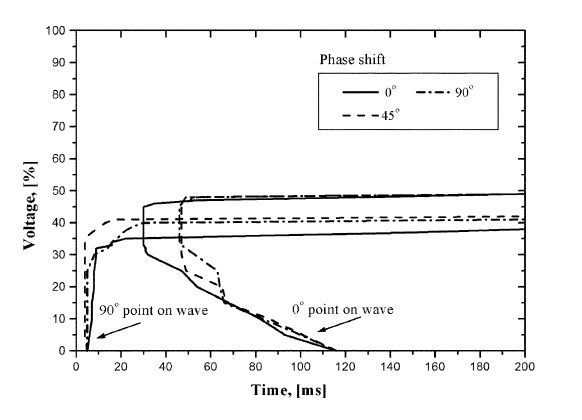
\includegraphics[width=0.8\linewidth]{../1/contactor}
		\caption[Contactor sag curves]{Contactor sag curves}
		\label{fig:contactor}
	\end{figure}
	%TODO: Add some more intro
	
	\section[Previous work]{Previous work} An attempt towards estimating trip probability for non-rectangular sensitivity curves have been undertaken in 
	%TODO: Add ref to Milanovic's work
	.The sensitivity curve was divided into a set of linear regions , and the trip probability was estimated based on the location of sag points on it.  
\end{document}

